\chapter{Experimental results}

% computer -> dds
%          -> scope
%          -> trigger
%          <- scope


% network analyzer (frequency dependence amplification)
% chirp signal deviation from ideal

\section{Intensity Control}
% test of long time stability

\begin{figure}[h]
  \centering
  \captionsetup{width=.8\textwidth}
  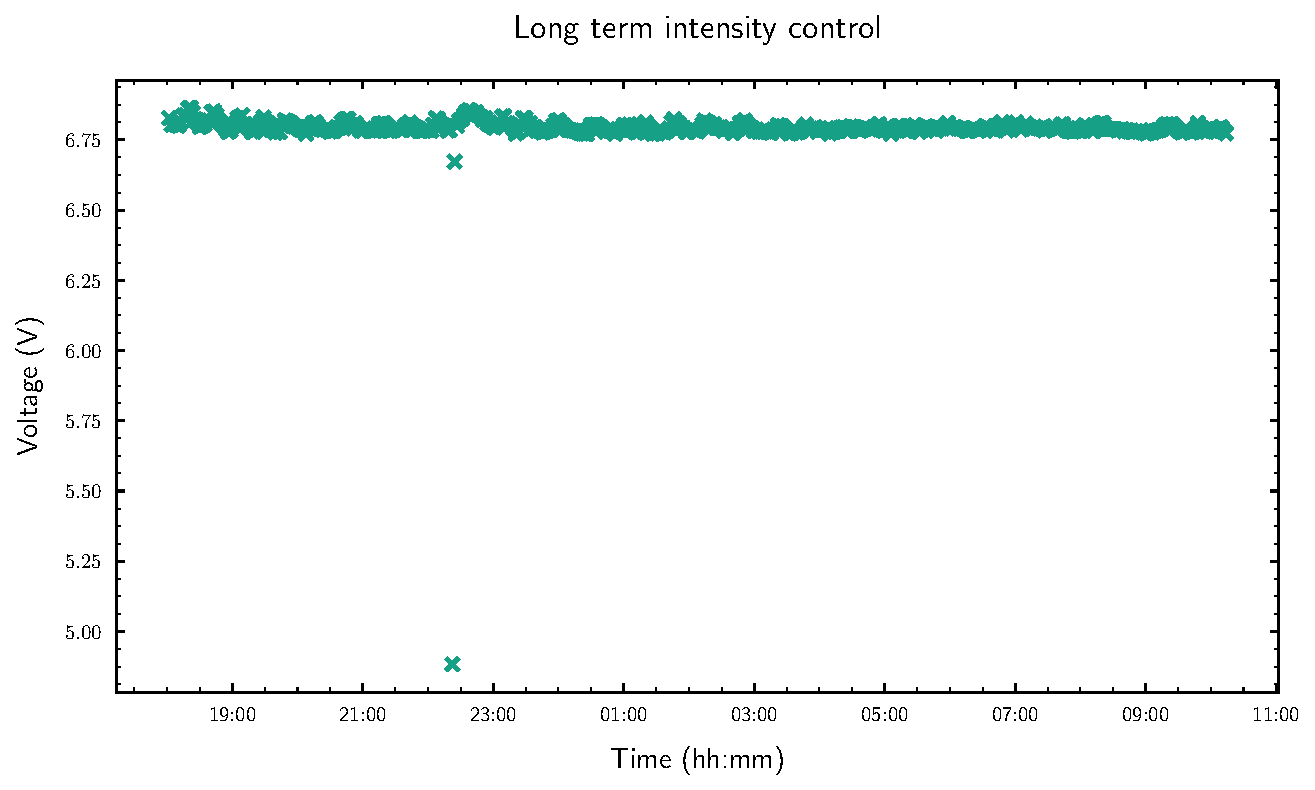
\includegraphics[width=\textwidth]{\figuredir{intensity/control-long.pdf}}
  \caption{Long measurement of the intensity without any electro-optics every
  \SI{130}{\second} for over \SI{16}{\hour} to determine the accuracy of the
  intensity controller. The outlier at around 23:00 were caused by a late
  laboratory visit.}
\end{figure}

\begin{figure}[h]
  \centering
  \captionsetup{width=.8\textwidth}
  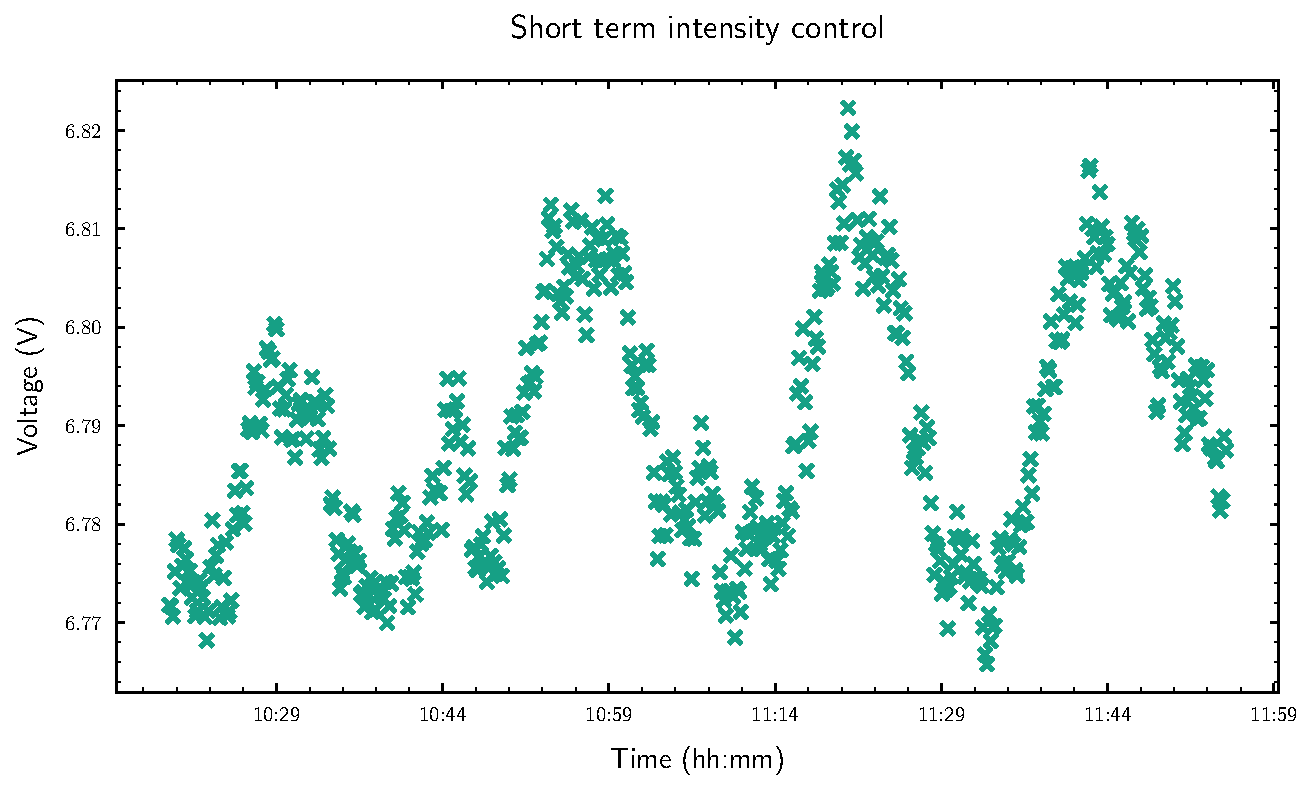
\includegraphics[width=\textwidth]{\figuredir{intensity/control-short.pdf}}
  \caption{Short measurement of the intensity without any electro-optics every
  \SI{10}{\second} for over \SI{1}{\hour} to determine the accuracy of the
  intensity controller.}
\end{figure}

\section{Synthesizer}

\begin{figure}[h]
  \centering
  \captionsetup{width=.8\textwidth}
  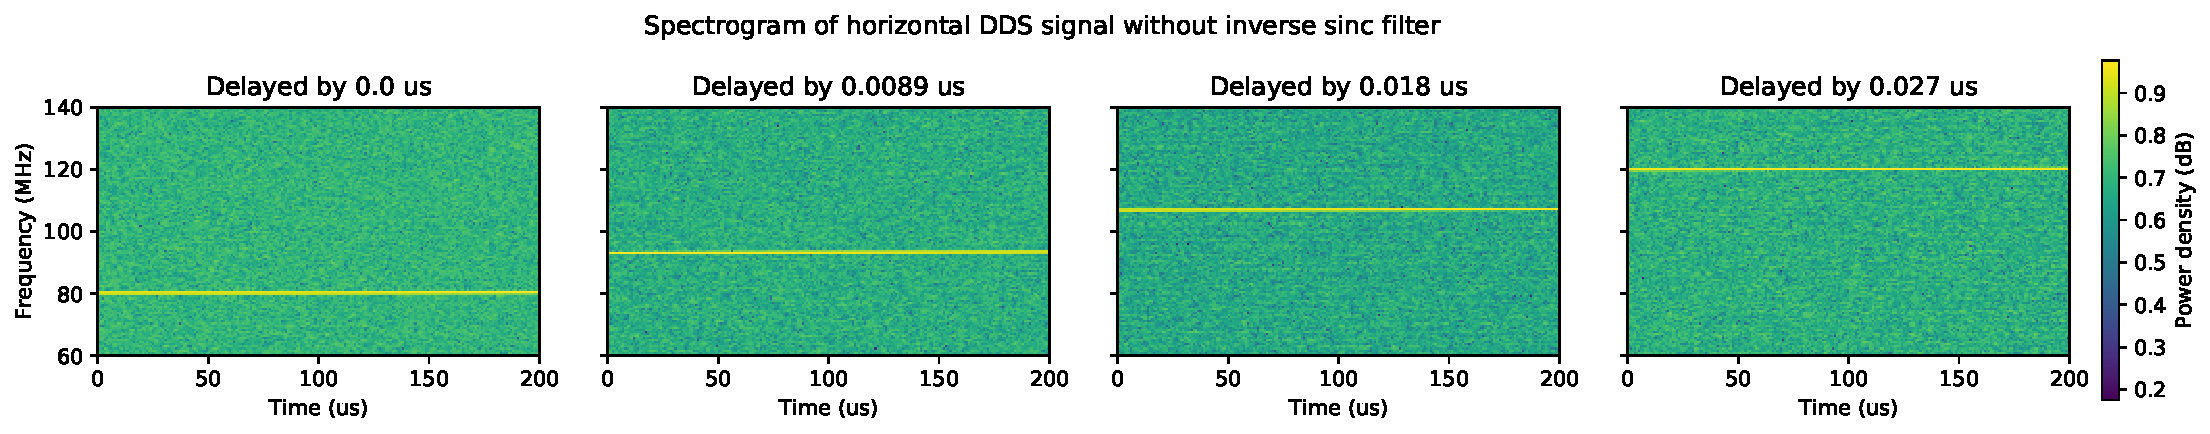
\includegraphics[width=\textwidth]{\figuredir{synthesizer/specgram.pdf}}
  \caption{Short measurement of the intensity without any electro-optics every
  \SI{10}{\second} for over \SI{1}{\hour} to determine the accuracy of the
  intensity controller.}
\end{figure}

\begin{figure}[h]
  \centering
  \captionsetup{width=.8\textwidth}
  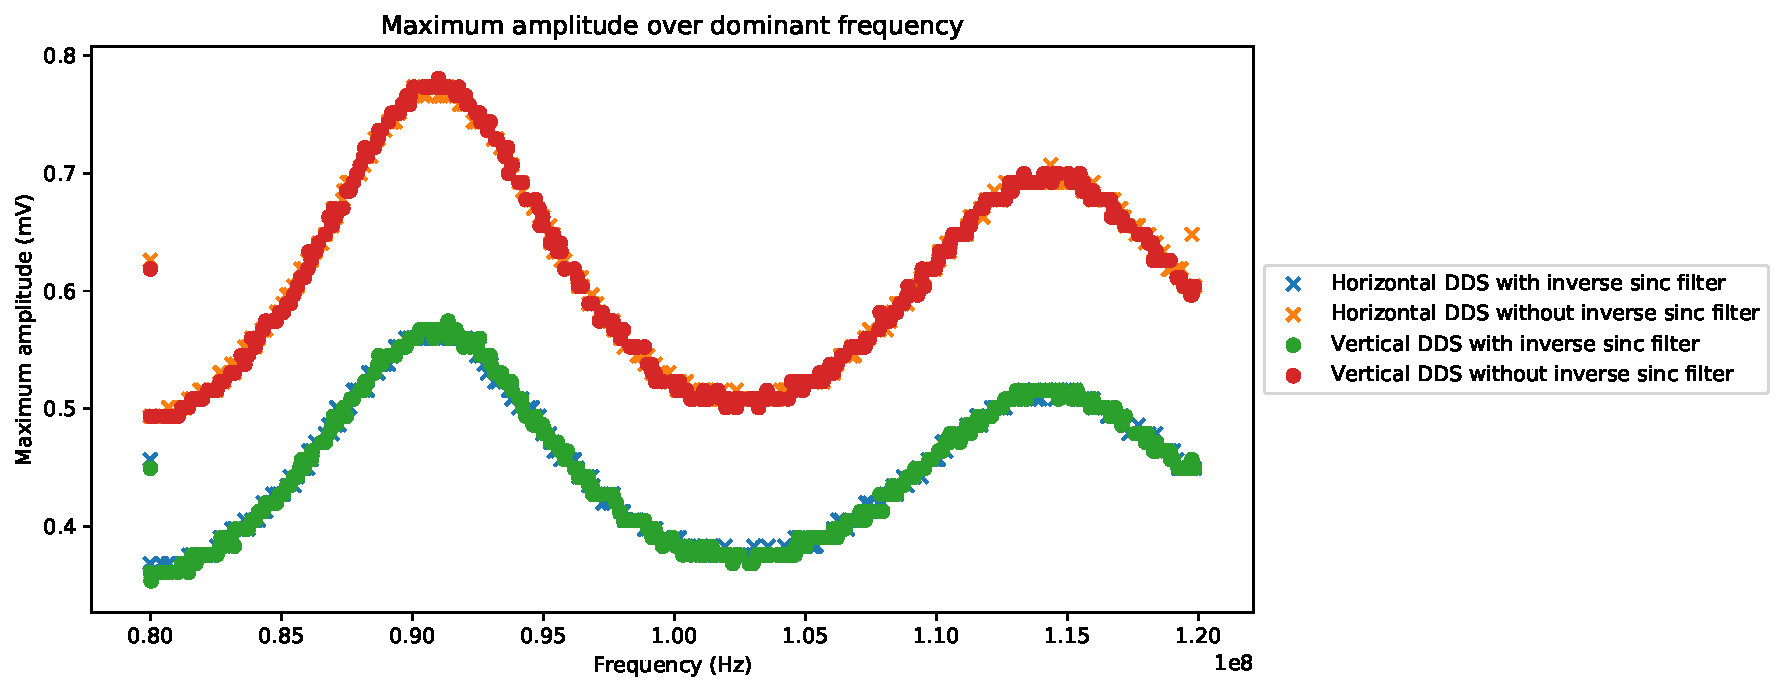
\includegraphics[width=\textwidth]{\figuredir{synthesizer/frequency.pdf}}
  \caption{Short measurement of the intensity without any electro-optics every
  \SI{10}{\second} for over \SI{1}{\hour} to determine the accuracy of the
  intensity controller.}
\end{figure}

\section{Amplifier}

\section{Acousto-optic deflector}
\subsection{Power matching}

\subsection{Intensity}
% H removed, V sweep (H in V position, vice versa)
% V removed, H sweep (V in H position, vice versa)

% H constant with V sweep
% V constant with H sweep

\chapter{Intensity Optimization}
\
% at different amplitude values
% without amplitude modulation
% with amplitude modulation
